% CVPR 2025 Paper Template; see https://github.com/cvpr-org/author-kit

\documentclass[10pt,twocolumn,letterpaper]{article}
\usepackage{amsmath}

%%%%%%%%% PAPER TYPE  - PLEASE UPDATE FOR FINAL VERSION
% \usepackage{cvpr}              % To produce the CAMERA-READY version
% \usepackage[review]{cvpr}      % To produce the REVIEW version -- hides authors
\usepackage{cvpr}  % To produce the CAMERA-READY version    
% \usepackage[pagenumbers]{cvpr} % To force page numbers, e.g. for an arXiv version

% Import additional packages in the preamble file, before hyperref
%
% --- inline annotations
%
\newcommand{\red}[1]{{\color{red}#1}}
\newcommand{\todo}[1]{{\color{red}#1}}
\newcommand{\TODO}[1]{\textbf{\color{red}[TODO: #1]}}
% --- disable by uncommenting  
% \renewcommand{\TODO}[1]{}
% \renewcommand{\todo}[1]{#1}



% It is strongly recommended to use hyperref, especially for the review version.
% hyperref with option pagebackref eases the reviewers' job.
% Please disable hyperref *only* if you encounter grave issues, 
% e.g. with the file validation for the camera-ready version.
%
% If you comment hyperref and then uncomment it, you should delete *.aux before re-running LaTeX.
% (Or just hit 'q' on the first LaTeX run, let it finish, and you should be clear).
\definecolor{cvprblue}{rgb}{0.21,0.49,0.74}
\usepackage[pagebackref,breaklinks,colorlinks,allcolors=cvprblue]{hyperref}

%%%%%%%%% PAPER ID  - PLEASE UPDATE
\def\paperID{*****} % *** Enter the Paper ID here
\def\confName{CVPR}
\def\confYear{2025}

\title{Final Project Report: Python-based JPEG-like Compression System}

\author{
Nicolas Drager, Muhammad Elarbi, George Roudebush\\
Department of Electrical and Computer Engineering\\
Northeastern University\\
\texttt{\{drager.n, elarbi.m, roudebush.g\}@northeastern.edu}
}

\begin{document}
\maketitle
\begin{abstract}
    This report presents a modular, Python-based JPEG-like image compression system developed for the course project in EECE 5698: Visual Sensing and Computing. The implementation supports a full compression and decompression pipeline, including image preprocessing, RGB-to-YCbCr color space conversion, customizable downsampling, fixed-size block division, Discrete Cosine Transform (DCT), quantization, entropy encoding via Huffman tables, and corresponding inverse operations. 
    
    To facilitate flexible experimentation, the system utilizes YAML-based configuration files that allow users to modify compression parameters such as quality factor, block size, and downsampling strategy. Parameter sweeps and semantic classification tests were conducted to evaluate tradeoffs between compression efficiency, processing time, and semantic preservation. Raw image input support and modular code structure enable advanced use cases, making the framework suitable for both academic exploration and practical testing.
    
    Although inspired by the JPEG standard, the system introduces configurable elements and detailed analysis tools to better understand compression behaviors. This report adheres to the CVPR-style conference paper format, as required by the course, despite being an academic project submission rather than a formal publication.
    \end{abstract}
        
\section{Introduction}
\label{sec:intro}

Image compression plays a vital role in modern visual communication systems, enabling efficient storage and transmission of large volumes of image data. From digital photography and medical imaging to web services and embedded systems, effective compression algorithms are crucial for managing bandwidth and storage constraints. Especially with the dawn of machine learning and in particular image classification, the need for reducing image sizes while retaining the general perceptual quality, has become even more apparent.

In modern visual systems, image compression enables efficient handling of visual data through two fundamental approaches. \textbf{Lossy compression} techniques like JPEG achieve significant size reduction by strategically discarding perceptually redundant information through its multi-stage pipeline of color space conversion (RGB to YCbCr), chrominance subsampling, block-based DCT transformation and quantization, and (in itself lossless) entropy coding \cite{haines1992compression,jpegOverview2025}. Modern successors like WebP and AVIF build upon these principles with enhanced predictive coding. In contrast, \textbf{lossless compression} methods such as PNG and FLIF preserve every bit of original data through DEFLATE compression and advanced context modeling respectively \cite{flif2016}, making them indispensable for medical imaging or archival purposes where fidelity is paramount. While JPEG's fixed configuration limits customization, newer but unfortunately still unpopular formats like JPEG XL \cite{jpegxl} can be seen as versatile alternatives that unify both lossy and lossless approaches while adding features like HDR support and progressive decoding.

\noindent In this project, we address the limitations of standard JPEG compression - particularly its rigid configuration that restricts parameter experimentation - by developing a \textbf{modular, Python-based image compression framework}. Inspired by JPEG's core architecture but designed for academic exploration, in particular regarding image classification, our system implements the traditional transform coding pipeline while exposing key variables for analysis, such as block size, quantization strategy, and downsampling rate. 

We further extended the project by incorporating parameter sweeps and classification-based evaluation, enabling both qualitative and quantitative assessments of compression performance. The primary goals of this work were to (1) build a working JPEG-like compression and decompression system from the ground up, (2) understand and visualize the effects of different parameter choices on output quality and file size, and (3) test whether compressed images preserve semantic content in machine-learning-based classification tasks. Our system design was partially inspired by recent advances in semantic-aware image compression~\cite{semanticDiffusion2023}.

%Regarding the mathematical notation, we use bold upper-case letters to denote arrays \(\bm{A}\), bold lower-case letters to denote vectors \(\bm{v}\), whereas scalars as plain \(s\).

The remainder of this paper is organized as follows: Section 2 describes our system implementation, Section 3 presents experimental results and analysis, and Section 4 offers concluding remarks.
The full source code and configuration files for this system are available at: \url{https://github.com/Roude/EECE5698-image-compression-roud-drag-elar}.

\section{Implementation}
\label{sec:implementation}

Our Python-based JPEG-like compression system is designed with modularity and experimentation in mind. It mirrors key stages of the classical JPEG pipeline while allowing for customized configurations through YAML files. In this section, we describe the architecture and underlying algorithms for each major component of our system, which include preprocessing, block-based Discrete Cosine Transform, quantization, entropy encoding, and full decompression support.

\subsection{Overall Compression Pipeline Structure}
The compression process consists of the following sequential stages:
\begin{enumerate}
    \item \textbf{Image Initialization}: Loading the configuration, the image, and ensuring the right format of the latter
    \item \textbf{Color Conversion}: Transforming the RGB image into YCbCr
    \item \textbf{Chrominance Downsampling}: Downsampling the two chrominance channels depending on configuration
    \item \textbf{Block Processing}: Channels get split into blocks, to each of them the following is applied
    \begin{enumerate}
    	\item \textbf{Discrete Cosine Transform (DCT)}: Transforming spatial pixel values to frequency domain.
		\item \textbf{Quantization}: Reducing frequency resolution based on configurable quantization tables.
    \end{enumerate}
    \item \textbf{Entropy Encoding}: Lossless entropy-encoding of block coefficients to compress data
        \begin{enumerate}
    	\item \textbf{Zigzagging}: Flattening the blocks
    	\item \textbf{Delta Encoding}: Take the differences of DC coefficients
    	\item \textbf{Run-Length Encoding}: Shortening AC component Array 
    	\item \textbf{Huffman Encoding}: Finding and encoding data with minimum length code 
    \end{enumerate}
    \item \textbf{File Encoding}: Encodes data and header into binary file, collects metrics
\end{enumerate}
\noindent
The decompression process reverses each of these steps.
\noindent
Each of the above steps is parameterized through YAML configuration files. Users can adjust quality settings, block sizes, quantization levels, and downsampling rates to generate different compression schemes.

\subsection{Image initialization}
\label{sec:initialization}
First, the configuration, if one has been provided either during initialization or calling of the image compressor object, is loaded, overwriting the default parameters.
Then the image gets loaded using the \texttt{scikit-image} library, unless it is a raw image file like CR2 in which case the loading is handled by using the \texttt{rawpy} wrapper for the \texttt{LibRaw} library.

Following the initial loading, all but the RGB channels get removed, since JPEG compression, with the exception of JPEG XL does not handle those. Furthermore, in case the channels have values outside of the 8 bit range (0 to 255), those get normalized and converted to unsigned integer 8 bit values per channel.

Thus, if we let  \(\bm{x} = (x,y)^T\) denote pixel coordinates, 
where $x \in \{0, \dots, w-1\}$ and $y \in \{0, \dots, h-1\}$, we now have the following RGB image $I$ which maps $\bm{x}$ to intensity values:
\[
I_{\text{RGB}}(\bm{x}) = \big( R(\bm{x}),\, G(\bm{x}),\, B(\bm{x}) \big) \in \{0, \dots, 255\}^3.
\]
Here each element of \( I(x, y) = (R(x,y), G(x,y), B(x,y)) \) contains three 8-bit unsigned integers, which are the RGB channels and are forwarded to color conversion.

\subsection{Color Conversion}
\label{sec:color}
JPEG's lossy compression relies to a good extent on downsampling the chrominance of an image. This is done as human vision is less sensitive to color variations than to brightness variations, and will therefore not perceive the downsampling of colors as much, while saving a lot of space.
To enable the chrominance downsampling, however, we first need to differentiate the luminance and chrominance parts of the images. This is done by converting RGB images to the YCbCr color space:
\begin{equation}
I_{\text{RGB}}(\bm{x}) = \begin{bmatrix} Y(\bm{x}) \\ Cb(\bm{x}) \\ Cr(\bm{x}) \end{bmatrix}
\end{equation}
\begin{equation}
= \begin{bmatrix} 0.299 & 0.587 & 0.114 \\ -0.1687 & -0.3313 & 0.5 \\ 0.5 & -0.4187 & -0.0813 \end{bmatrix} \begin{bmatrix} R(\bm{x}) \\ G(\bm{x}) \\ B(\bm{x}) \end{bmatrix} + \begin{bmatrix} 0 \\ 128 \\ 128 \end{bmatrix}
\end{equation}

\subsection{Downsampling}
To downsample the resulting YCbCr image, the chrominance channels are processed as follows depending on a downsampling factor  $d \in \mathbb{N}^+$. 
If \(d > 1\), a running average is put into place for each of the two chrominance channels, only taking every \(d\)-th pixel in such a way that the dimensions of the resulting \(\tilde{Cb}\) and \(\tilde{Cr}\) are as follows. 
\[
(h_c, w_c) = \left( \left\lceil \frac{h}{d} \right\rceil, \left\lceil \frac{w}{d} \right\rceil \right)
\]
These are then rounded to integers and put in a python list together with the unchanged Y channel. It obviously doesn't make sense anymore to represent the image as a regular array, instead they are being treated as 3 arrays in a python list.

If \(d = 1\), or in other words downsampling is not to be applied, it will just return the YCbCr channels in a list, to save computation time instead of doing an identity operation.
It is important to note that this is different than how downsampling is executed in the JPEG standard. 
With JPEG compression, the downsampling is performed by keeping individual pixels values in a pattern.
This is done with speed, rather than accuracy or quality in mind. 
For small downsample factors, keeping individual pixel values and averaging nearby pixels does essentially the same thing, but we are also interested in the compression behavior when downsample factors become very large, at which point there will be a noticeable difference between individual pixels and average pixel downsampling approaches.

\subsection{Block Processing}
To go from here, each channel is divided into usually square non-overlapping blocks using the block size parameter \(b \in \mathbb{N}^+\) (e.g. 8 is used in standard JPEG, ours is configurable). In cases where \(h \mod b \neq 0\) or \(w \mod b \neq 0\) for either the regular or the chrominance dimensions, the blocks will not be square, which is something that needs to be accounted for later. 

\subsubsection{Discrete Cosine Transformation}
First, the unsigned 8 bit integer blocks are converted to signed 16 bit integers, while getting centered to zero by subtracting 128.

Then, an orthonormal type II 2D Discrete Cosine Transformation (DCT), which is a real-valued offshoot of the Discrete Fourier Transformation (DFT), is applied to each block using the following formula:

\begin{align}
  &F(u, v) = \frac{1}{\sqrt{N*M}} C(u)C(v) \\ \sum_{x=0}^{N} \sum_{y=0}^{M} f(x,y)
  &\cos\left( \frac{(2x+1)u\pi}{2N} \right) \cdot \cos\left( \frac{(2y+1)v\pi}{2M} \right)
\end{align}

where $C(k) = \frac{1}{\sqrt{2}}$ if $k = 0$ and $C(k) = 1$ otherwise. The two axes (x and y) have their own respective sum indicies because our compression pipeline tolerates images with lengths and widths in pixels not divisible by the block size. This leaves results in some of the blocks being rectangular, so the axes need to be dealt with separately. Because the block represents only a small portion of the image, which usually includes very little varriation across the block, most of the image energy is usually concentrated into the upper-left lower-frequency corner of the DCT block.

Our implementation hereby leverages \texttt{scipy.fftpack.dct} for speed and numerical accuracy.

\subsubsection{Quantization}
Quantization now discards high-frequency DCT coefficients in each block, by dividing element-wise with a previously configured quantization matrix $Q \in \mathbb{N}^{b\times b}$. This is done to reduce the amount of less information carrying, nonzero components which makes Run-Length-Encoding later on much more effective. It should be noted that different quantization matrices are used for luminance and chrominance, with the latter usually receiving harsher quantization. Each coefficient $F(u,v)$ is divided by a quantization matrix $Q(u,v)$ and rounded:

 %Skipping of higher-frequency basis functions often leads to so-called blocking artifacts, but also ringing is observed particularly in case of image edge structures.

\begin{equation}
F_Q(u,v) = \left\lfloor \frac{F(u,v)}{Q(u,v)} + 0.5 \right\rfloor
\end{equation}

If the block dimensions do not match the dimensions of the quantization matrix, because of it being part of the lower or right border of the image with the image dimension not being divisible with \(b\), the block gets padded with zeros until it reaches them.

The highest-frequency component is principally set to zero to avoid issues with the zigzagging algorithm later on.

\begin{equation}
	F_Q(b-1,b-1) = 0
\end{equation}

The JPEG quantization matrix values are highly tuned and optimized across a range of quality factor for 8x8 blocks.
However, because one of the goals of this projects is to understand compression characteristics across a range of bloc sizes, we need to be able to generate quantization parameters that quantize a similar portion of the matrix for a range of block sizes. 
Because of this, we implemented two different functions that generate quantization matrix values from a small set of parameters.
\begin{itemize}
    \item \textbf{Baseline JPEG-style}: A scaled standard luminance matrix.
    \item \textbf{Quarter-Gauss-Distribution}: Tighter control on high frequencies.
    \item \textbf{LN-Norm}: Control over mid-range frequencies and their quantization level relative to high and low frequency component quantization.
    \item \textbf{Custom sweep}: Users can specify arbitrary YAML matrices.
\end{itemize}

\subsubsection{Quarter-Gauss-Distribution Quantization}

The so called "Quarter Gauss" quantization matrix function generates a quantization matrix of size NxN, using three parameters: The block size ($N$), the max quantization value ($A$), and the standard deviation ($\sigma$).

Let $d_{ab}$ be the L2 norm distance of a matrix entry $M_{ab}$from matrix element $M_{NN}$.

Then each element of the quantization matrix can be generated as shown in figure \ref{fig:gaussian_quant}

\begin{figure}
	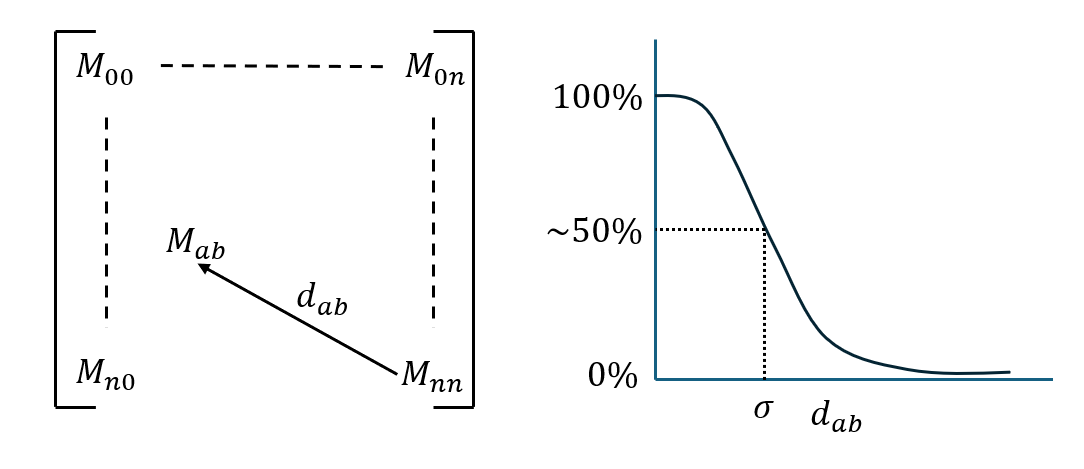
\includegraphics[width=0.5\textwidth]{assets/Quarter Gauss Quantization.png}
	\caption{Visual representation of the "Quarter Gaussian" quantization parameters.}
	\label{fig:gaussian_quant}
\end{figure}
% \begin{equation}
% 	\label{eq:gaussian_quant}
% 	M_{ab} = \frac{A}{2\pi\sigma^2}e^{-\frac{d_{ab}^2}{2\sigma}} 
% \end{equation}

\subsubsection{LN-Norm}

Gaussian distribution of quantization values gives us fine control over the structure of the quantization matrix, but in the spirit of exploration, we also implemented an LN-Norm function for generating the quantization matrices.
The LN-norm of two points is defined in equation \ref{eq:ln_norm}

\begin{equation}
D_{ab, N} = ((x_a - x_b)^N + (y_a - y_b)^N)^{(1/N)}
\label{eq:ln_norm}
\end{equation}

Choosing $N\in[1,2]$ will result central elements in the quantization matrix being closer to the top left, so those frequencies will be quantized less aggressively. Choosing $N\in[2,\inf]$ will result in mid-range frequencies being quantized more similarly to the high frequency elements. 
A visualization of these effects is shown in figure \ref{fig:LN-norm}.

\begin{figure}
	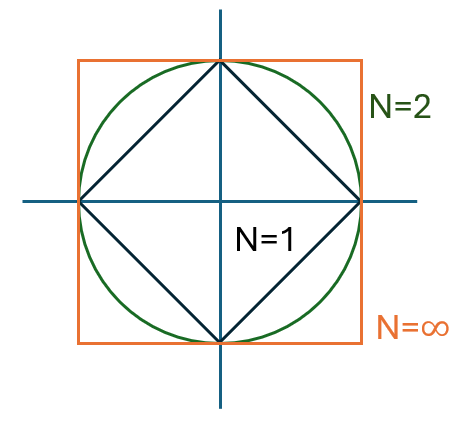
\includegraphics[width=0.5\textwidth]{assets/LN-Norm.png}
	\caption{Visualization of LN-Norm for all possible N values. lines represent unit distance from the origin under the chosen N-normalization.}
	\label{fig:LN-norm}
\end{figure}
Quality can be tuned directly or indirectly via configuration files in \texttt{compression\_configurations/\allowbreak quantization\_sweep/}.

\subsection{Entropy Coding}
The quantized channels are now transferred to the entropy coding method, where they are again broken up into blocks. If they are not \(\in \mathbb{N}^{b\times b}\), they again get padded with zeroes. They are then flattened to be \(z \in \mathbb{N}^{1\times b^2}\) 1D arrays using an algorithm called zigzag ordering, which utilizes following a previously initialized zigzag pattern, to rearrange the frequency values in such a way that bundles lower frequency values in the front as seen below.

\begin{figure}[H]
	\centering
	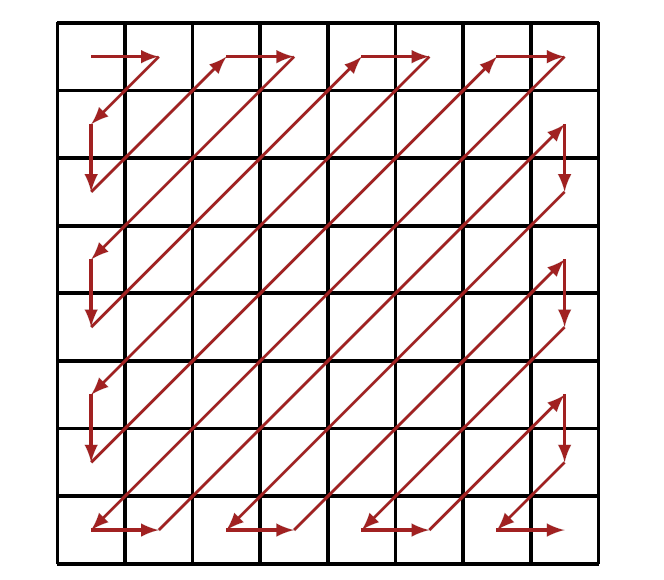
\includegraphics[width=0.8\linewidth]{assets/zigzag.png}
	\caption{Rearrangement of a \(8\times8\) block using zigzag pattern}
	\label{fig:zigzag}
\end{figure}

Then, as lower frequency values usually carry most information and energy, the so called DC component \(z_0 = F_Q(0,0)\) of each block is extracted and the difference is made with its predecessor from the block prior, in order to reduce the dynamic range of the DCT coefficients. This is called delta encoding, and the DC values are treated and even encoded differently from the remaining so called AC components. It is to be noted that luminance and chrominance values are separated here as elsewhere.

The AC components \(z_1,...,z_{b^2-1})\) are now forwarded to a method called run-length encoding, which for every value \(z_i \neq 0, i \in {1,...,b^2-1}\) returns a tuple as follows, given an array \(Z = [z_1, \ldots, z_{b^2-1}]\):

\begin{equation*}
	\mathcal{R}(Z) = \begin{cases}
		(z_i, c_i) & \text{for } a_i \neq 0 \text{ with } c_i \text{ preceding zeros} \\
		(0,0) & \text{if only zeroes remaining in the block}
	\end{cases}
\end{equation*}


\begin{algorithm}
	\caption{Run-Length Encoding Algorithm}
	\label{alg:jpeg-rle}
	\begin{algorithmic}[1]
		\Require $\text{zigzag\_array} = [z_1, \ldots, z_n]$
		\Ensure List of $(value, zero\_count)$ tuples with EOB marker
		
		\State $\text{encoded} \gets \emptyset$
		\State $\text{zero\_count} \gets 0$
		\For{each element $a_i \in \text{zigzag\_array}$}
		\If{$z_i = 0$}
		\State $\text{zero\_count} \gets \text{zero\_count} + 1$
		\Else
		\State $\text{encoded.append}((a_i, \text{zero\_count}))$
		\State $\text{zero\_count} \gets 0$ \Comment{Reset counter after non-zero value}
		\EndIf
		\EndFor
		\State $\text{encoded.append}((0, 0))$ \Comment{Add End-of-Block (EOB) marker}
		\State \Return $\text{encoded}$
	\end{algorithmic}
\end{algorithm}

Since the number of zeroes is concentrated in the end after the zigzag ordering, the returned array contains only a few tuples, which however are enough to describe the whole block. Since \(F_Q(b-1,b-1) = 0\) earlier, we do not need to worry about the \((0,0)\) EOB potentially elongating the block to be longer than its maximum size when decoding.


\subsubsection{Huffman Encoding}

\textbf{This Section Needs Citations}
Both the AC and the delta-encoded DC values of all blocks are finally forwarded, separated both by AC and DC as well as by luminance and chrominance, to the Huffman encoding algorithm. Here each symbol is counted and thus has its frequency determined. This frequency shall axiomatically serve as the probability of a symbol \(p(x_i)\) from now on.

Huffman encoding is a widely used lossless data compression algorithm that assigns variable-length codewords to symbols based on their probabilities. The key idea is to use shorter codes for more frequent symbols and longer codes for less frequent ones, minimizing the average codeword length. To further understand Huffman encoding, we first need some basic concepts from information theory. 
The information content of a symbol \( x_i \) with probability \( p(x_i) \) is defined as:
\[
I(x_i) = \log_2 \left( \frac{1}{p(x_i)} \right) = -\log_2 p(x_i).
\]
This measures how surprising or informative an event is: the less probable the symbol, the higher its information content.
The entropy \( H(X) \) of an information source is the expected (average) information content:
\[
H(X) = -\sum_{i=1}^{n} p(x_i) \log_2 p(x_i).
\]
Entropy represents the minimum average number of bits required to represent each symbol from the source.
From Shannon's Source Coding Theorem, the minimum expected codeword length \( L_{\text{min}} \) for a symbol \( x_i \) satisfies:
\[
H(X) \leq L_{\text{avg}} < H(X) + 1,
\]
where \( L_{\text{avg}} \) is the average length of the codewords. Huffman encoding achieves near-optimal compression, with \( L_{\text{avg}} \) very close to \( H(X) \).
Huffman encoding does this by constructing a prefix-free binary code (no codeword is a prefix of another) ensuring unambiguous decoding, using the following steps:
\begin{enumerate}
	\item \textbf{Frequency Calculation:} Compute the frequency (or probability) of each symbol in the input.
	\item \textbf{Priority Queue:} Build a min-heap where each node represents a symbol and its frequency.
	\item \textbf{Tree Construction:}  
	\begin{itemize}
		\item Repeatedly extract the two nodes with the smallest frequencies.
		\item Merge them into a new internal node with their combined frequency.
		\item Assign '0' to the left branch and '1' to the right branch.
		\item Reinsert the new node into the heap.
	\end{itemize}
	\item \textbf{Code Assignment:} Traverse the tree from the root to each leaf, recording the binary path to generate the Huffman code for each symbol.
\end{enumerate}

After the codewords were assigned for each group of values (Lum DC, Lum DC, Chrom DC, Chrom AC) and thus the so-called Huffman tables are created, the channels are iteratively encoded using the respective Huffman table, resulting in a long bitstream, which contains the data of the image. This alongside the Huffman tables themselves is forwarded to file encoding.

The benefit of using four different huffman tables instead of just one, is that the data often looks very different for each group, making it at least in most cases more efficient to use. However due to having multiple codewords for a recurring symbol, the header becomes larger.

Standard JPEG actually uses fixed Huffman tables instead, which is less compression efficient but definitely faster to encode.

Despite the fact that Huffman coding is basically optimal in terms of average word length, there are methods that provide even better compression such as arithmetic coding and asymmetric numeral systems (ANS). Arithmetic coding encodes data as a single fractional number, allowing symbols to occupy fractional bits and tightly approaching entropy limits. ANS improves on this by using integer-state transformations for similar compression gains while being computationally faster. Both methods excel where Huffman struggles, e.g. with highly skewed distributions (like 99 percent probable symbols), since they avoid Huffman's requirement of whole-bit codewords. Arithmetic coding is even used in JPEG XL, but due to patent issues in the 80s does not enjoy high popularity. For our project, we opted for Huffman coding, as it is not only easier, but because we believe that the focus of the work should lie on the lossy part of the compression and its impact on image classification.
\subsection{File Encoding}
The file encoding method handles the final stage of our image compression pipeline, packaging all compressed components into a proprietary binary file format using our initials (.rde). The process begins by preparing the compression metadata - it converts the Huffman code tables and quantization matrices into JSON-serializable formats while preserving the original settings. The actual compressed bitstream (previously generated through Huffman encoding) gets processed into a byte-aligned format, with padding bits added if needed to complete the final byte.

The output file follows a specific structure: first a 4-byte header length indicator, followed by the JSON header containing all decompression parameters (quantization tables, Huffman dictionaries, image dimensions, and padding information), and finally the packed binary data representing the compressed image content. Alongside the binary file, the function generates comprehensive compression metrics including detailed size breakdowns (separating header overhead from actual image data), processing timings, and quality measurements like compression ratio and bits-per-pixel. These metrics get saved to a companion JSON file and can optionally be displayed in a formatted table, providing insights into the compression efficiency and the relative contributions of different components to the final file size. The implementation maintains careful byte-level control throughout the packaging process while handling all necessary data conversions between Python objects, JSON structures, and raw binary formats.
\subsection{Decompression Pipeline}
Decompression reverses all previous stages, while stripping the data of padded zeroes:
\begin{enumerate}
	\item \textbf{File Decoding}: Read binary data and extract header/metadata (quantization tables, Huffman codes, etc.) which are used in the later methods
	\item \textbf{Entropy Decoding}:
	\begin{itemize}
		\item \textbf{Huffman Decoding}: Reconstruct DC/AC coefficients
		\item \textbf{Run-Length Decoding}: Expand compressed AC coefficients
		\item \textbf{Delta Decoding}: Reverse DC coefficient differences
		\item \textbf{Inverse Zigzag}: Reshape 1D array to 2D frequency blocks
	\end{itemize}
	\item \textbf{Block Processing}:
	\begin{itemize}
		\item \textbf{Dequantization}: Multiply coefficients by quantization table values
		\item \textbf{IDCT}: Convert frequency-domain blocks to spatial pixels
	\end{itemize}
	\item \textbf{Chrominance Upsampling}: Upsample Cb/Cr channels if downsampled
	\item \textbf{Color Conversion}: Convert YCbCr back to RGB
	\item \textbf{Image Finalization}: Clamp pixel values, save image
\end{enumerate}
The decompression logic is implemented in \texttt{src/decompression.py}. It was in many cases quite challenging to get the correct output; especially block placement was a point of contention at first.

One point of interest here might be the handling of the upsampling. Before the colors can be converted back to RGB, the lower dimension chrominance channels need to be expanded accordingly. This can be done using any way of interpolation, we decided on nearest-neighbor for computation speed. However linear and other interpolation algorithms can be used to get better results.

\subsection{Evaluating Compression Distortion}

In order to evaluate compression distortion, two metrics are used: Structrual Similarity Index (SSIM) and PSNR (Peak Signal to Noise Ratio). These metrics are commonly used to compare "ground truth" images to processed images. \cite{wang2004image}\cite{psnr} The skimage package included as part of SciPy includes functions to calculate both SSIM and PSNR for a pair of images. These metrics are systematically evaluated across a sweep of images.

\subsection{Evaluation of Semantic Information}

While JPEG and other compression algorithms where designed largely with aesthetic quality preservation in mind, an important metric for modern compression algorithms is the preservation of semantic information. 
Evaluating the Semantic Preservation of a compression algorithm is essentially asking \enquote {Does the compressed image produce the same classification result with the same model input parameters?}. A competing requirement for compression performance is compression ratio, or the fraction of image data the compressed encoded image takes up. As the compression ratio approaches zero, it's expected that the semantic content of the image would be lost. Therefore, understanding what compression parameters improve compression rate without degrading semantic content is the subject of exploration for this next section.

We propose Confidence Error as a general summary metric for Semantic Preservation. Let $C_{err}$ represent our metric, the Confidence Error. Let $L_{max}$ be the highest probability label from and inference pass with ResNet50 on the uncompressed image. Let $P^{Lmax}_{uncompressed}$ be the probability of this label. Let $P^{Lmax}_{compressed}$ be the classification probability of label $L_{max}$ on the compressed image.

$$
\textrm{C}_{err} = \frac{\|P^{Lmax}_{uncompressed} - P^{Lmax}_{compressed}\|}{P^{Lmax}_{uncompressed}}
$$

When performing parameter sweeps across various compression parameters, we evaluate Confidence Error with the following algorithm
\begin{algorithm}
    \label{alg:Confidence Error Algorithm}
    \caption{Evaluating Confidence Error during compression parameter sweeps}
	\begin{algorithmic}[1]
    \Require{ Reference image $I_{ref}$, compressed image $I_{cmp}$, pretrained model $Res50$}
    \Ensure{ $C_{err}$ for the two images}
	\State $I_{ref, pp}$ = preprocess($I_{ref}$)
	\State $W_{ref \ outputs}$ = $Res50$.infer($I_{ref, pp}$)
	\State $P_{ref \ classes}$ = softmax($W_{outputs}$)
	\State $L_{max}$ = argmax({$P_{ref classes}$})
	\State $P^{Lmax}_{uncompressed}$ = $P_{classes}$[$L_{max}$]
	\State $I_{cmp, pp}$ = preprocess($I_{comp}$)
	\State $W_{comp \ outputs}$ = $Res50$.infer($I_{cmp, pp}$)
	\State $P_{cmp \ classes}$ = softmax($W_{outputs}$)
	\State $P^{Lmax}_{compressed}$ =  $P_{cmp \ classes}$[$L_{max}$]
	\State $\textbf{return}\ \frac{P^{Lmax}_{uncompressed} - P^{Lmax}_{compressed}}{P^{Lmax}_{uncompressed}}$
	\end{algorithmic}
\end{algorithm}

%TODO: Add Description of preprocessing and classification for ResNet50 to Implementation Section.

In this way, the semantic content is systematically compared and evaluated for each of the test images.

\subsubsection{Image Preprocessing for ResNet50}

ResNet50 requires images to be passed in cropped to a size of 224x224, and normalized to a pixel value range per channel of approximately -1 to 1. In order to avoid unfavorable crops of images, each image scalled down to a height of 256, and then center-cropped to 224x224 pixels. This way, a large portion of the center of the image is passed into the classifier. It is worth noting that this resize and crop preprocessing is essentially a lossy compression before the semantic information is extracted. If the only purpose of an compression algorithm is to extract semantic information, and the visual quality is of no concern, likely the most effective way to compress that image would be to downsample the image uniformally to the required size and perform a lossless encoding from there. There are many cases however, where the aesthetic quality of the image is important, and for these, the full image resolution is needed.

\subsection{Configuration Management}
\label{sec:config_management}
All compression parameters are stored in human-readable YAML files. These files are passed into the system via CLI (e.g., \texttt{results\_compression.py --config homemade\_compression\_jpeg\_like.yaml}).

Sweeps are conducted using \texttt{test/parameter\_sweeps.py}, which iterates over YAML directories for block sizes, downsampling levels, and quantization schemes.

Additional configuration directories (e.g., \texttt{quantization\_sweep\_chroma/}, \texttt{quantization\_sweep\_luma/}, \texttt{quantization\_sweep\_small\_blocks/}) were created during final testing to support more granular sweep control over chroma and luma quantization matrices.

\subsection{Implementation Highlights}

The repository is structured as follows:
\begin{itemize}
    \item \texttt{src/}: core pipeline (compression, decompression, utilities)
    \item \texttt{compression\_configurations/}: parameter sweep YAMLs
    \item \texttt{test/}: experimental evaluation, sweeps, classification
    \item \texttt{assets/}: test images
\end{itemize}

The test image suite was recently expanded and reorganized to support broader variation in content and file types. New naming conventions (e.g., \texttt{subject\_*}, \texttt{landscape\_*}) and formats (including TIFF, AVIF, PNG, and high-resolution RAW CR2) enable more granular benchmarking of compression behavior across diverse scenes, lighting conditions, and semantic content.

Key implementation goals included:
\begin{enumerate}
    \item Enabling experimentation with minimal code changes
    \item Supporting multiple image formats (PNG, JPG, AVIF, WEBP, CR2)
    \item Using only Python and standard packages (\texttt{numpy}, \texttt{PIL}, \texttt{scipy}, etc.)
    \item Support for advanced quantization experiments, including Quarter Gaussian and L-N norm-based matrices, with separate control over luminance and chrominance channels
\end{enumerate}

\subsection{Division of Work}
\label{sec:division-of-work}

While the initial division of work outlined in our February project proposal was tentative, the responsibilities naturally evolved during development. Although all team members collaborated conceptually, the division of work is outlined below:
\begin{itemize}
  \item George Roudebush: compression pipeline, parameter sweeps, quantization table and function development, baseline JPEG comparison, Semantic Preservation method development and testing, utility methods, test image dataset curation, and configuration integration, report results section, production of datasets for report and analysis of those datasets.
  \item Nicolas Drager: Entropy encoding, file coding, decompression pipeline, size estimation and compression metrics in file coding, bug fixes in all other compression methods, making it possible to switch between parameters, utility methods, huffman methods, testing methods, adapting the introduction in the report, implementation report up to \ref{sec:config_management}
  \item Muhammad Elarbi: decompression pipeline, padding error fixes, unit test development, raw image test dataset creation (CR2), output location handling, final-report drafting, documentation, and code cleanup
\end{itemize}
\section{Results}
\label{sec:results}

This section presents an evaluation of our JPEG-like compression system across multiple parameter sweeps and test scenarios. The goal is to assess compression performance with respect to visual quality, file size, semantic preservation, and runtime efficiency.

\subsection{Overview of Evaluation Goals}
Our evaluation focuses on the following:
\begin{itemize}
    \item \textbf{Compression Quality}: Comparison of output image quality under various compression settings
    \item \textbf{Compression Ratio}: Size reduction achieved with each configuration
    \item \textbf{Semantic Preservation}: Classification consistency of compressed images using pre-trained models
    \item \textbf{Runtime Performance}: Timing analysis for compression and decompression operations
\end{itemize}

\subsection{Test Methodology}
Experiments are conducted using YAML configurations across:
\begin{itemize}
    \item \texttt{compression\_configurations/\allowbreak quantization\_sweep/}
    \item \texttt{compression\_configurations/\allowbreak downsample\_sweep/}
    \item \texttt{compression\_configurations/\allowbreak block\_size\_sweep/}
    \item \texttt{compression\_configurations/\allowbreak quantization\_sweep\_chroma/}
    \item \texttt{compression\_configurations/\allowbreak quantization\_sweep\_luma/}
    \item \texttt{compression\_configurations/\allowbreak quantization\_sweep\_small\_blocks/}
\end{itemize}

Each configuration is tested on a standardized dataset of images (\texttt{assets/test\_images/}) with various formats and content types. Results are logged in corresponding metrics files (.metrics.json) and visual artifacts are stored in \texttt{results/}.

These additional sweeps were introduced after the initial draft to better isolate compression artifacts and parameter sensitivity across chroma and luma components.

To assist with analysis and visualization, we created a dedicated Jupyter notebook (\texttt{notebooks/plot\_results.ipynb}) to plot trends in PSNR, SSIM, compression ratios, and runtime performance across different sweep parameters.

\subsection{Parameter Sweeps}

To test the sensitivity of our various metrics across a variety of compression parameters, the following parameter sweeps are performed:

\begin{table}[h!]
    \centering
    \caption{Gaussian Quantization Weights Quantization Parameters Tested}
    \begin{tabularx}{0.5\textwidth}{X c c c}
        \toprule
        \ & \textbf{Luma} & \textbf{Chroma} \\
        \ & \textbf{Quantization} & \textbf{Quantization} \\
        \ & \textbf{Max, $\sigma$} & \textbf{Max, $\sigma$} \\
        \midrule
        No Quantization & 1 , 1 & 1, 1 \\
        High Quality & 10,3 & 20, 3 \\
        Quality & 30, 5 & 40, 5 \\
        Moderate Quality & 60, 6 & 75, 6 \\
        Low Quality & 100, 8 & 125, 8 \\
        Very Low Quality & 150, 10 & 200, 10 \\
        \bottomrule
    \end{tabularx}
    \label{tab:Quantization-Parameters-Table}
\end{table}

\begin{table}[h!]
    \centering
    \caption{LN-Norm Quantization Parameters Tested}
    \begin{tabularx}{0.5\textwidth}{X c c c}
        \toprule
        \ & \textbf{Luma} & \textbf{Chroma} \\
        \ & \textbf{Quantization} & \textbf{Quantization} \\
        \ & \textbf{Max, Min} & \textbf{Max, Min} \\
        \midrule
        No Quantization & 1 , 1 & 1, 1 \\
        L1.5 High Quality & 10, 5 & 20, 10 \\
        L1.5 Quality & 40, 20 & 50, 30 \\
        L1.5 Med Quality & 50, 20 & 60, 30 \\
        L1.5 Low Quality & 100, 30 & 125, 40 \\
        L1.5 Very Low Quality & 200, 80 & 150, 60 \\
        L2 High Quality & 10, 5 & 20, 10 \\
        L2 Quality & 40, 20 & 50, 30 \\
        L2 Med Quality & 50, 20 & 60, 30 \\
        L2 Low Quality & 100, 30 & 125, 40 \\
        L2 Very Low Quality & 200, 80 & 150, 60 \\
        L3 High Quality & 10, 5 & 20, 10 \\
        L3 Quality & 40, 20 & 50, 30 \\
        L3 Med Quality & 50, 20 & 60, 30 \\
        L3 Low Quality & 100, 30 & 125, 40 \\
        L3 Very Low Quality & 200, 80 & 150, 60 \\
        \bottomrule
    \end{tabularx}
    \caption{Quantization Parameters for Gaussian Quantization Sweeps. Max is the quantization value in the bottom left entry of the quantization matrix, and sigma is the width parameter for the gaussian curve which defines the rest of the entries in the matrix. See \ref{fig:gaussian_quant} for more detail.}
    \label{tab:Quantization-Parameters-LN-Norm}
\end{table}

\begin{table}[h!]
    \centering
    \caption{Downsample Rates Tested, No further quantization}
    \begin{tabularx}{0.5\textwidth}{X c c c}
        \toprule
        \ & \textbf{Downsample Rate} \\
        \midrule
        No Quantization & 1 \\
        High Quality & 2 \\
        Quality & 4 \\
        Moderate Quality & 6 \\
        Low Quality & 8 \\
        Very Low Quality & 12 \\
        \bottomrule
    \end{tabularx}
    \label{tab:Downsample Parameters}
\end{table}

\begin{table}[h!]
    \centering
    \caption{Block sizes tested, Gaussian Weight Quantization, max 50, $\sigma = $ block size/2}
    \begin{tabularx}{0.5\textwidth}{X c c c}
        \toprule
        \ & \textbf{Block Size} \\
        \midrule
        High Quality & 4 \\
        Quality & 8 \\
        Moderate Quality & 16 \\
        Low Quality & 24 \\
        Very Low Quality & 48 \\
        \bottomrule
    \end{tabularx}
    \label{tab:Block Size Sweep}
\end{table}

\subsection{Compression Quality}

By comparing SSIM and PSNR to Compression Ratio allows us to determine which compression parameters can be modified to reduce image size while maintaining image quality.

\subsubsection{JPEG Baseline}

As a starting point of comparison, JPEG baseline images are evaluated across a range of quality factors. As expected, both quality metrics look better with higher quality factors, shown by figure \ref{fig:psnr_jpeg} and figure \ref{fig:ssim_jpeg}.
There also appears to be a loose correlation between PSNR and compression ratio shown in figure \ref{fig:psnr_vs_compression_ratio}. Generally for any given image as the compression ratio decreases, so does the PSNR. However, when looking at a wide variety of images, the quotent of the PSRN to the compression rate can be very different image to image.

\begin{figure}
    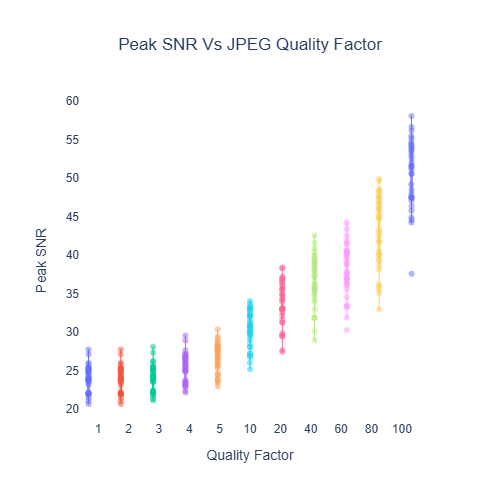
\includegraphics[width=0.5\textwidth]{assets/JPEG Quality Factor and PSNR.png}
    \caption{Quality factor vs PSNR}
    \label{fig:psnr_jpeg}
\end{figure}

\begin{figure}
    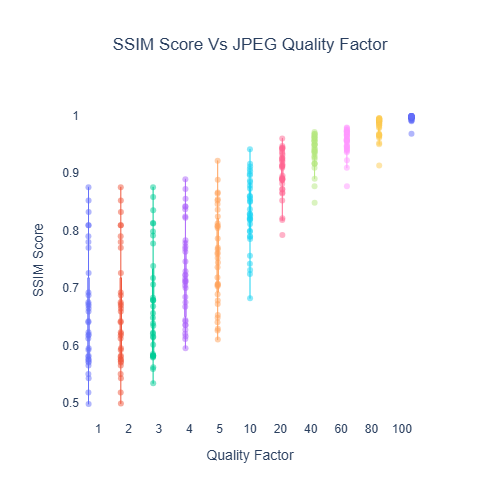
\includegraphics[width=0.5\textwidth]{assets/JPEG Quality factor and SSIM Score.png}
    \caption{Quality Factor vs SSIM}
    \label{fig:ssim_jpeg}
\end{figure}

\begin{figure}
    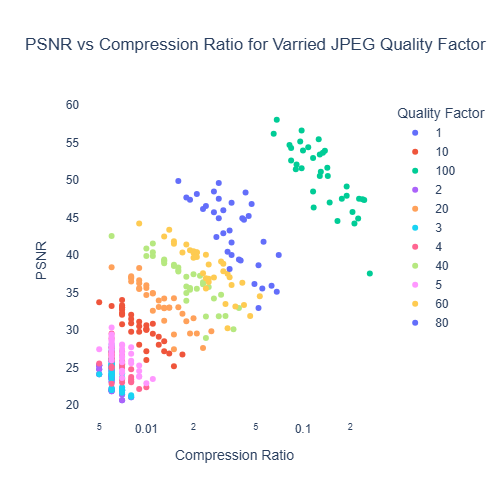
\includegraphics[width=0.5\textwidth]{assets/JPEG Compression Ratio Vs PSNR.png}
    \caption{PSNR Vs Compression Rate for a variety of Quality Factors}
    \label{fig:psnr_vs_compression_ratio}
\end{figure}

\subsubsection{Compression Quality Vs Quantization}

Using our flexible compression framework, quantization is varied according to table \ref{tab:Quantization-Parameters-Table} and \ref{tab:Quantization-Parameters-LN-Norm}. These quantizations are applied to images with an additional 2x chrominance downsampling applied to them.

Interestingly, when compraing compression ratio to PSRN, there is a clear bifurcation as the quantization rate increases. Some images experience a clear increase in PSNR as the compression rate is increased, consistent with the results from the JPEG baseline. However, many of the images see hardly any increase in PSRN as the compression ratio increases \ref{fig:gauss_quantization_vs_psnr}. Taking a closer look at these images, it appears that the images for which PSRN does not correlate to compression ratio are the high or very high quality images in the dataset, with dimensions on the order of \~ 6000 x 4500. Since for all quantizations, there is a chrominance downsample factor applied, for these large images, this is likley the cause of the degrated PSNR. For images with smaller starting dimensions, a 2x chromiance downsample factor does not remove as much information, so it's expected that the PSNR would not be as degraded.

\begin{figure}
    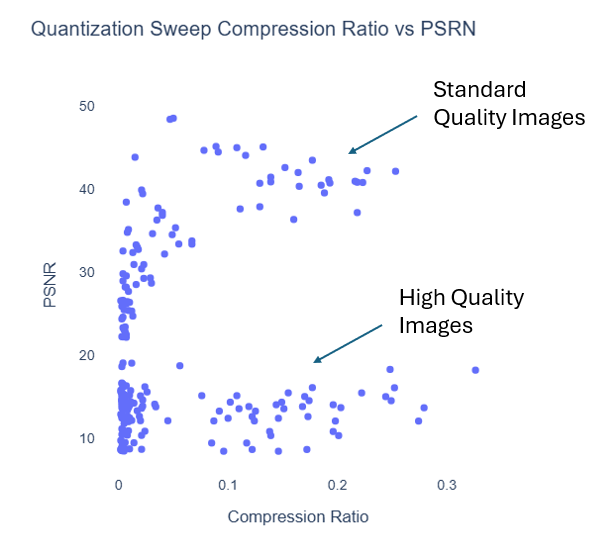
\includegraphics[width=0.5\textwidth]{assets/Quantization Sweep Compression Ratio vs PSRN.png}
    \caption{PSRN vs Compression Ratio across a sweep of quantizations defined in table \ref{tab:Quantization-Parameters-Table}. Clear bifurcation shows that images with larger starting dimensions suffer more from even a modest 2x chrominance downsample factor}
    \label{fig:gauss_quantization_vs_psnr}
\end{figure}

\subsubsection{LN-Norm Quantization}

Along with having the ability to fine-tune the exact quantization parameters, our flexible compression pipeline also gives the ability to generate quantization matricies with different structures. Here we evaluate if the relative quantization of mid-range frequences relative to high and low frequencies can help improve performance without resulting in additional file size. Unfortunately, there is little to no change in the relationship between PSNR and compression rate as the norm N is varied, or even comprared to the Gaussian Weight quantization, as shown in figure \ref{fig:LN-norm_quantization_performance}

\begin{figure}
    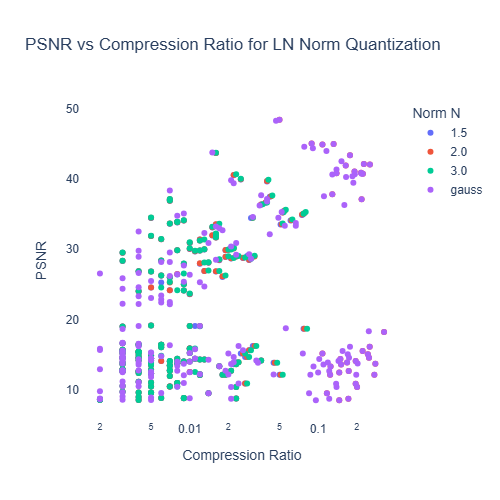
\includegraphics[width=0.5\textwidth]{assets/PSNR for LN Quantization with gaussian weights.png}
    \caption{PSRN vs compression ratio for a variety of quantization weights. Changing the relative rates of quantization for mid-range frequencies has no impact on the relationship between the image PSNR and the compression rate.}
    \label{fig:LN-norm_quantization_performance}
\end{figure}

In addition to there being very little change in the compression ratio, LN-normalized images look visible more degraded, as shown in figure \ref{fig:quantization_function_comparison}

\begin{figure}
    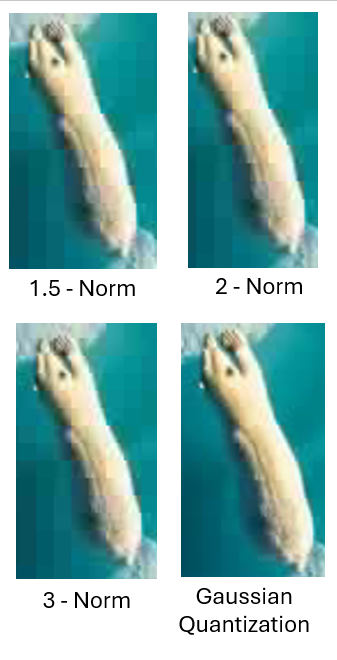
\includegraphics{assets/Quantization Function Comparison.png}
    \caption{LN-norm quantization results compared to Gaussian Quantization weights}
    \label{fig:quantization_function_comparison}
\end{figure}

\subsubsection{Chrominance Downsampling}

JPEG leverages a YCbCr colorspace in order to distinguish between Luminance and Chrominance information in the image.
This distinction allows for the Chrominance Channels to be downsampled while the Luminance stays full rank.
In this section we analyze the effects of downsampling on our compressed image quality metrics. 
Shown in figure \ref{fig:downsample_vs_psnr}, downsampling uniformly reduces PSNR and compression rate. However, unlike Quantization, image quality drops off steeply and compression rate does not improve significatly for large downsample factors.

\begin{figure}
    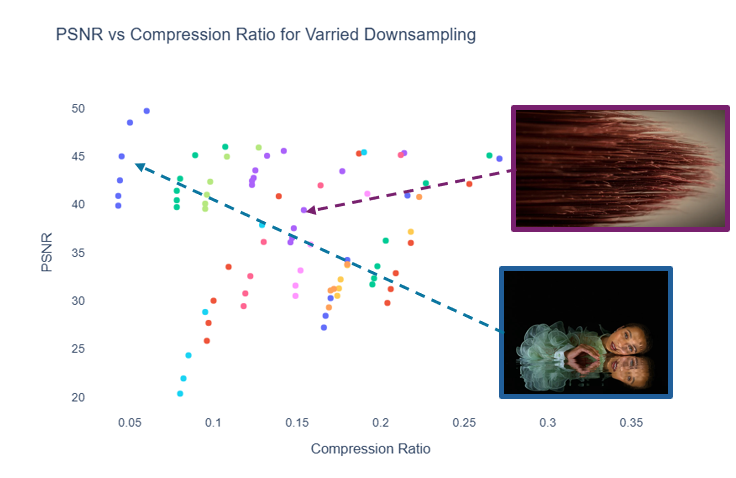
\includegraphics[width=0.5\textwidth]{assets/PSNR vs Chromiance Downsampling with Images.png}
    \caption{As expected, generally increasing the chromiance downsample rate (and therefore reducing the compression ratio), the PSRN metric is degraded.}
    \label{fig:downsample_vs_psnr}
\end{figure}

\subsubsection{Block Size}

For this experiment we vary the block size according to table \ref{tab:Block Size Sweep}. We find the larger blocks do not compress the images as much as small blocks \ref{fig:block_comp_rates}. Additionally, varrying the block size also does not see to effect the PSNR to a large extent. However, qualitatively the blocking strategies are visibly different \ref{fig:block_quantization_artifacts}. The effect of smaller blocks is that the edges of each block becomes more clearly visible, giving the effect that the entire image has been downsampled in 2x2 pixel blocks. In larger blocks, there are shimmers and other quantization artifacts which are visible across the block upon close inspection, despite the block edges being less obvious. It's clear that a small block with a reasonable compression rate, that preserves a gradient over the block while minimizing frequency quantization artifacts is ideal for image visual appeal.

\begin{figure}
    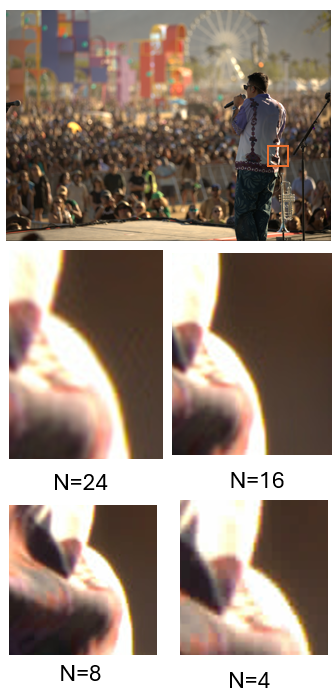
\includegraphics[width=0.5\textwidth]{assets/Block Quantization Artifacts.png}
    \caption{A visualization of block size artifacts. As blocks become larger, individual blocks have more detail, and features within the blocks are more clear, but block boundaries are still visible.}
    \label{fig:block_quantization_artifacts}
\end{figure}

\begin{figure}
    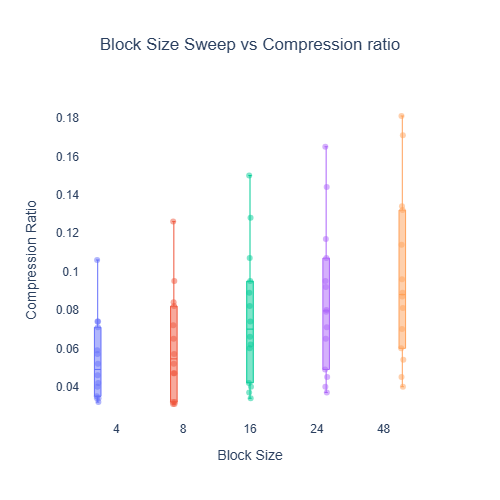
\includegraphics[width=0.5\textwidth]{assets/Comp Rate VS block Size.png}
    \caption{Compression Rates improve with smaller block sizes, while larger block sizes result in overall larger image size, despite the same relative quantization being applied across block sizes.}
    \label{fig:block_comp_rates}
\end{figure}

\begin{figure}
    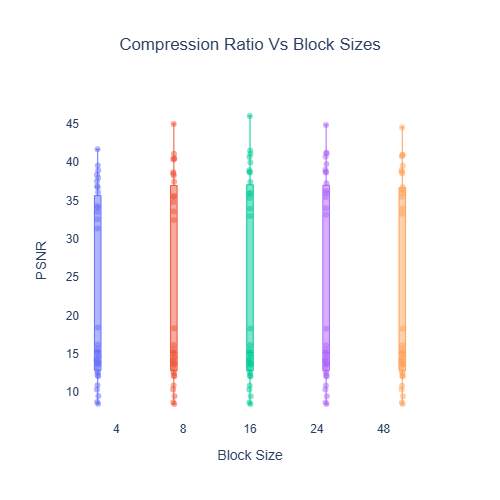
\includegraphics[width=0.5\textwidth]{assets/Block Size Vs PSNR.png}
    \caption{As block size is varried with quantization kept relativly the same, the PSNR does not change.}
\end{figure}

\subsubsection{Compression Quality Discussion}

By far the most effective way to reduce image file size while maintaining high image quality metrics is to apply a moderately agressive quantization on relativly small blocks. In order for this quantization to be successful, high frequencies need to be heavily attenuated while low frequencies are maintained. Other modifications or factors swept either resulted in a very fast degradation of image quality with little change in compression ratio, or did not siginificantly effect either metric while introducing undesireable visual artifacts.

\subsection{Semantic Preservation}
Images were evaluated using a pre-trained classification model (e.g., ResNet50) to test whether compression degrades semantic content. This was done using \texttt{test/classification\_tests.py}.

\textbf{TODO: Replace charts in this section with ones that have clearer labels and axis titles.}

\subsubsection{Test Images for Semantic Preservation}

In order to evaluate our compression pipeline, a set of test images with a variety of objects for classification was chosen. 
Resnet50 is a model largely for objects and non-human subjects, so images with a clear subject well centered in the image, spanning range of sizes relative to the size of the image. 
Additionally, some images were deliberately chosen because they contain multiple subjects or subjects where the classification is somewhat ambiguous, to see if these are more adversely effected by the compression than clear images, see figure \ref{fig:test_images} for the continum of subjects tested. 
All test images are evaluated against all compression configurations. A set of novel images for classification are chosen for benchmarking rather than ImageNet or ResNet training set images to avoid compounding effects of muliple lossy compressions on the image. 
ImageNet and ResNet images are already JPEG images, and therefore have some (unknown) level of compression already applied to them. The test set images are either raw formats or lossless image formats (such as .png, and .webp).

\begin{figure}
    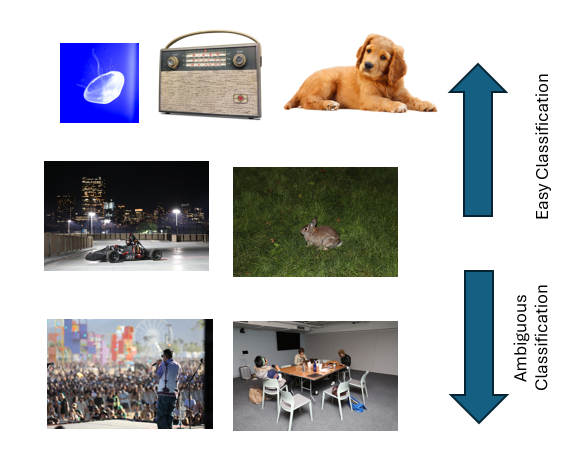
\includegraphics{assets/Classification Sweep.png}
    \caption{Images are chosen for classification with a variety of subjects and easy of classification.}
    \label{fig:test_images}
\end{figure}

\subsubsection{JPEG Compression as a baseline for Semantic Preservation}

As a natural starting point of comparison for Semantic Preservation, we evaluate the semantic preservation of the JPEG compression standard.
The JPEG standard only exposes a single compression parameter available for adjustment, the JPEG Quality Factor (QF) largly effects the quantization table values for each of the Descrete-Cosine-Transformed Blocks.
Images are evaluated for semantic preservation using algorithm \ref{fig:Annotated JPEG Baseline}.
Results are then parameterized by compression rate and original image content (figure \ref{fig:Comp vs Ratio JPEG Baseline}). There appears to be an inflection point around compression ratios of 0.1 or less, where certain images loose nearly all of their semantic content. For certain images, even ratios of 0.01 do not increase confidence error.

Taking a closer look at these images, images where the subject is large relative to the frame of the image have their semantic classifications more well preserved even with extremely agressive compression. However, When images contain other objects than the subject, or the subject of the image is small, the compression has a more dramatic impact on the classification. This trend is highlighted in figure \ref{fig:Annotated JPEG Baseline}

\begin{figure}
    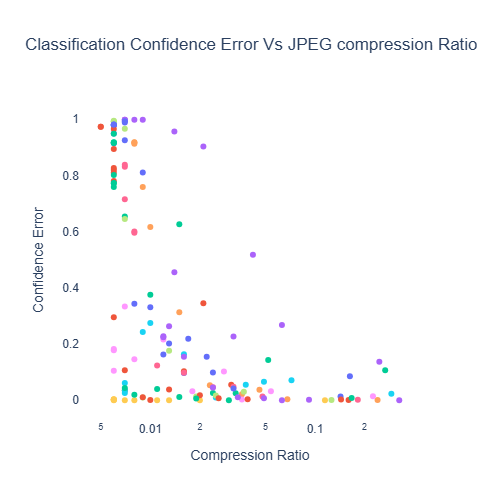
\includegraphics[width=0.5\textwidth]{assets/Baseline JPEG Confidence vs Comp Ratio.png}
    \caption{Confidence Error vs Compression Ratio for JPEG Compression. Smaller Values on the X axis correspond to smaller compressed images, while higher values on the Y axis correspond to a higher classification error rate. It appears that compression rates have little to no effect on semantic content until the compression ratio dips below 0.1.}
    \label{fig:Comp vs Ratio JPEG Baseline}
\end{figure}

\begin{figure}
    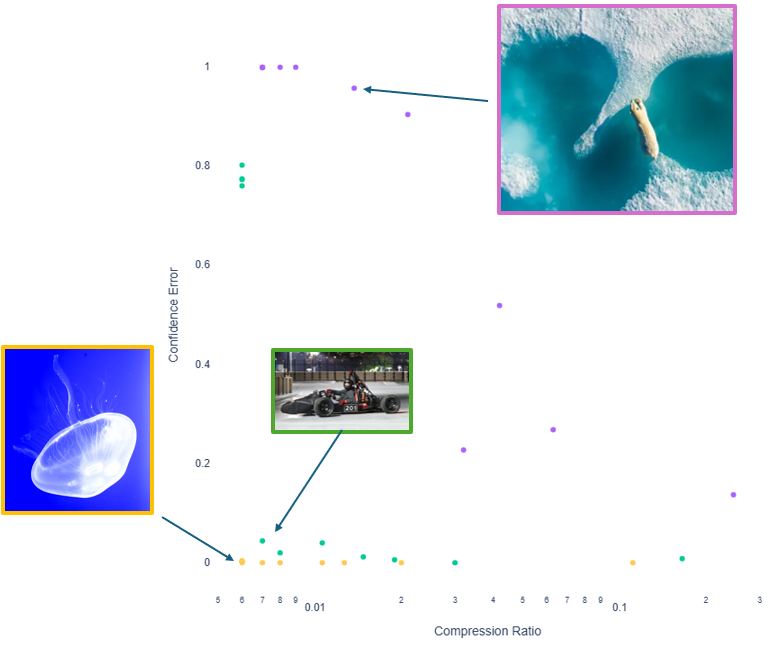
\includegraphics[width=0.5\textwidth]{assets/JPEG Baseline Compression with Examples}
    \caption{Certain Images have their semantic content preserved even with extremely agressive compression parameters where images are reduced to 0.6\% of their original size. Other images suffer from a sharp decline preserved semantic information. Intuitively, the higher the percentage of pixels in the image that represent the subject of classificatoin (as in the case of the jellyfish and the racecar), the better semantic preservation through compression.}
    \label{fig:Annotated JPEG Baseline}
\end{figure}

The results for JPEG compression on these test images can serve as a baseline for other compression parameters evaluated.

\subsubsection{Quantization Sweep Results}

One of the compression parameters that our flexible compression pipeline makes available are the Quantization Tables.
These can be generated using Gaussian of the bottom right distance or scaled min and max values by the L-N Norm distances.
When Quantization is increased, more of the high-frequency information of the image is lost, so by sweeping through a set of quantization parameters, we can demonstrate the relative sensitivity of semantic information on high vs low frequency components.
The flexible compression pipeline also enables setting of luminance and chrominance quantization seperately, so we can explore whether semantic information is more closely tied to Luminance, or Chrominance information.

The parameters for Chrominance and Luminance quantization tested are listed in table \ref{tab:Quantization-Parameters-Table}. For sweeps with just Luminance or just Chrominance varied, the other quantization channel is processed with no Quantization.
All experiments use a Chrominance downsample factor of 2.

Similar to the JPEG baseline, Confidence Error increases sharply when the compression rate drops below 0.1, as shown in figure \ref{fig:Confidence vs Quantization}
Interestingly however, when just the Chrominance or just the Luminance channels are varied, both the Confidence error and the compression ratio suffer. Shown in figure \ref{fig:just chroma or luma downsampling}
\begin{figure}
    \label{fig:Confidence vs Quantization}
    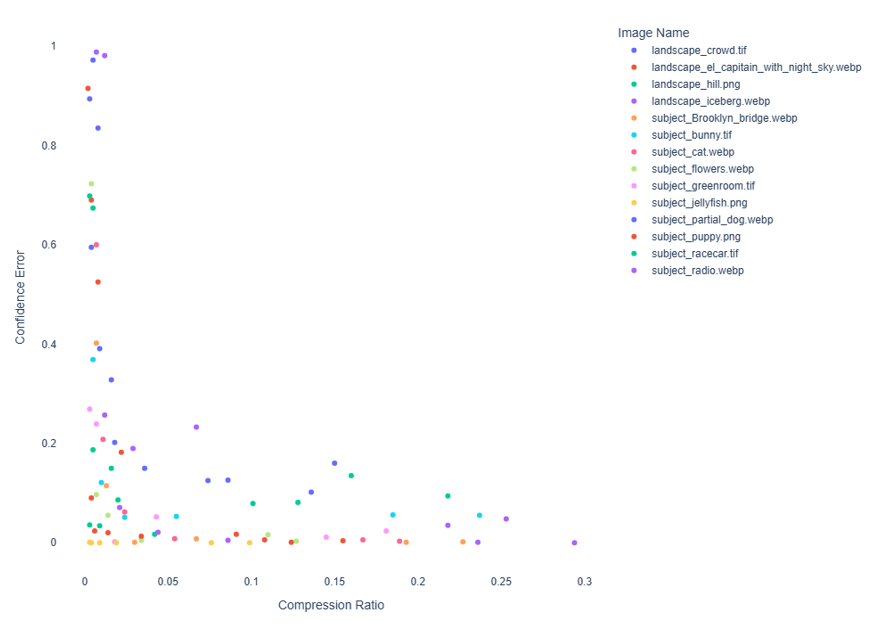
\includegraphics[width=0.5\textwidth]{assets/Quantization Sweep No Title Chrominance and Luminance.png}
    \caption{Confidence Error vs Compression Ratio as the Quantization parameters are varied. Quantization has very little effect on Semantic information until the compression ratio gets below approximately 0.1.}
    \label{fig:Confidence vs Quantization}
\end{figure}
\begin{figure}
    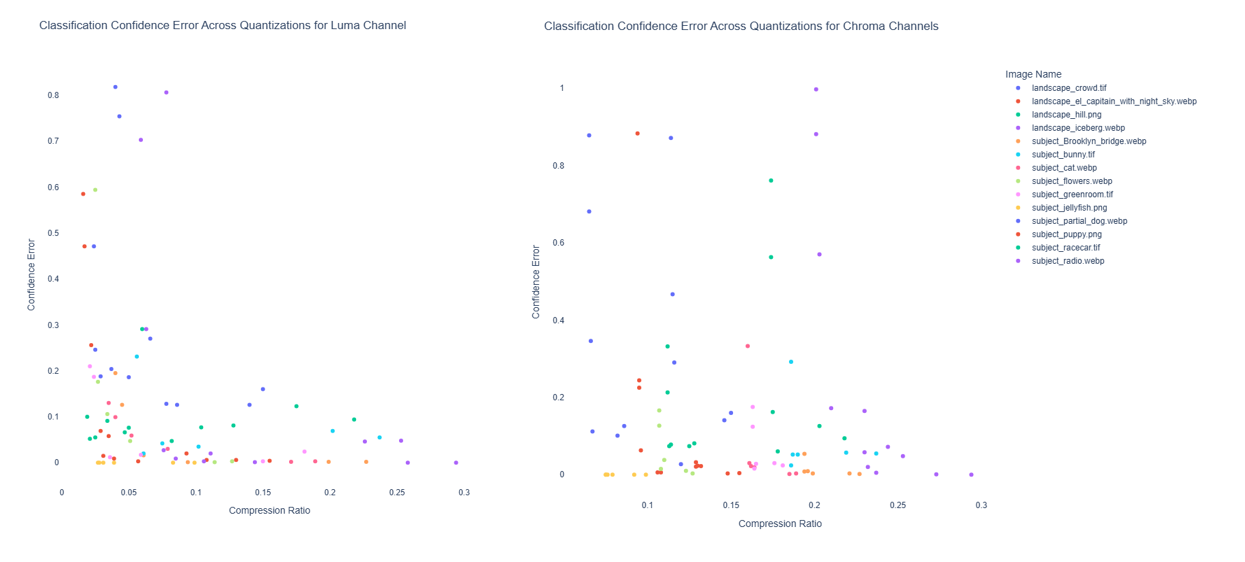
\includegraphics[width=0.5\textwidth]{assets/Chroma and Luma downsampling combined.png}
    \caption{Unlike in \ref{fig:Confidence vs Quantization}, if just one of the channel types is quantized, the semantic information is quickly lost, and the compression ratio is not improved.}
    \label{fig:just chroma or luma downsampling}
\end{figure}

\subsubsection{Block Size}

Block size affects the compressed result by changing pixel block base unit the Descrete Cosine Transform operates on.
Larger Blocks include a wider range of frequencies and more information being transformed each time, while smaller blocks allow for discontinuities at block edges to potentially go unnoticed.
In this experiment, we test apply our compression to images while varrying block size.

\begin{figure}
    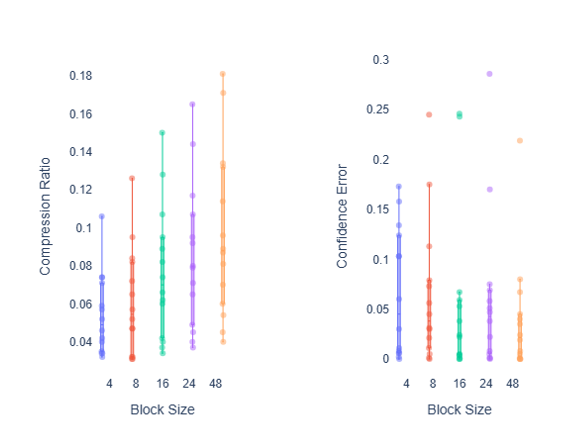
\includegraphics[width=0.5\textwidth]{assets/Confidence Err Vs Block Size.png}
    \caption{Confidence Error vs Compression Ratio for a variety of block sizes. As with other swept parameters, compression ratio and confidence error are inversely related.}
    \label{fig:block_size_sweep}
\end{figure}

\subsubsection{Discussion}

Similar to compression quality, among all tested parameters, quantization proved the most effective in reducing image file size while preserving semantic information. However, some other interesting trends arrise. If quantization is applied to only one of the channels, even if that is the chromiance chaannel only, the Confidence Error increases significantly over relativly modest Compression Ratios. This suggests that there is Semantic meaning encoded in color information in a different color space the YCbCr color. Future work could include applying different color transformations to the image before quantizing.

\subsection{Runtime and Performance}
Execution time for both compression and decompression is measured and stored during sweeps. Aggregate runtime plots can be shown here.

One main difference between our compression pipeline and JPEG compression is that the huffman tables are not pre-computed. Through our tests we note that this accounts for a significant portion of the computational load for compression and decompression \ref{fig:runtimes}. It is important to note that these runtimes are not comparable to well established codex standards, as most machines have dedicated hardware for performing these computations. The computed runtimes are only comparable to other internal results. 

\begin{figure}
    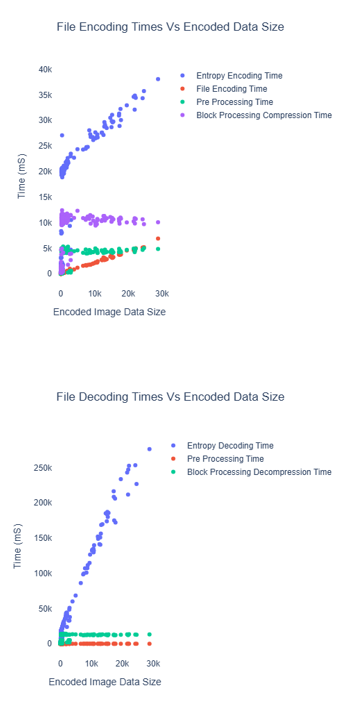
\includegraphics[width=0.5\textwidth]{assets/Runtimes Summary.png}
    \caption{Sets of sampled runtimes for the most computationally intensive parts of the our flexible compressoin pipeline.}
    \label{fig:runtimes}
\end{figure}


\section{Conclusion}
\label{sec:conclusion}

This project presents a modular, Python-based JPEG-like image compression system developed for EECE 5698: Visual Sensing and Computing. Our implementation emulates the classical JPEG compression pipeline while introducing key enhancements to promote experimentation and flexibility. By decoupling pipeline stages and supporting parameterized configuration files, our system allows users to explore the impact of various compression strategies (including downsampling factors, block sizes, and quantization levels) on image quality and file size.

We implemented every core stage of the compression and decompression workflow, including color space conversion, block-based DCT, configurable quantization, entropy encoding via a custom Huffman implementation, and a full-featured decompression pipeline. Throughout development, we prioritized technical rigor and reproducibility, carefully handling edge cases such as padding, alignment, and raw image format compatibility (e.g., Canon CR2). All major system parameters are exposed via YAML configuration files, which enable both one-off experiments and automated parameter sweeps. Supporting scripts like \texttt{results\_compression.py}, \texttt{parameter\_sweeps.py}, and \texttt{results\_decompression.py} were developed to streamline batch testing and metrics collection.

Initial evaluation of the system suggests promising results. While full testing is still underway at the time of writing, early sweeps demonstrate that the system behaves in line with theoretical expectations — increasing quantization severity yields smaller file sizes at the cost of quality, and chroma subsampling schemes like 4:2:0 result in noticeable color loss while preserving perceptual fidelity. A detailed analysis of these results, including compression ratios, PSNR, SSIM, runtime metrics, and semantic preservation scores, will be finalized and integrated into Section~\ref{sec:results}. Future updates to this paper should incorporate those results, along with any generated figures, graphs, or evaluation tables. We ask our team members leading testing efforts to append this section accordingly.

Beyond implementation fidelity, the system’s architecture serves as a useful sandbox for exploring compression tradeoffs. Unlike most off-the-shelf JPEG implementations, our system exposes every internal stage, allowing students and researchers to tune, visualize, and analyze the consequences of individual design decisions. This modularity makes it well-suited for further experimentation, including the integration of alternative transforms (e.g., wavelets), advanced quantization techniques, or perceptual encoding strategies such as saliency-aware masking.

Despite its strengths, the system has limitations. While sufficient for academic exploration, it is not optimized for real-time performance or production-scale workloads. Huffman table generation is fixed at encode-time based on a training set and lacks adaptive tuning. Error resilience and fault tolerance are minimal, and certain test images (especially large or atypically dimensioned files) may reveal edge case bugs. These limitations point to several promising areas for future work, such as:

\begin{itemize}
    \item \textbf{Adaptive Huffman tables} that update dynamically based on image content
    \item \textbf{Advanced entropy coding} (e.g., arithmetic coding or context modeling)
    \item \textbf{Support for progressive JPEG encoding}
    \item \textbf{Integration of perceptual metrics or machine learning-based tuning}
    \item \textbf{Visualization tools} for examining intermediate DCT coefficients, zigzag orderings, or compression artifacts
\end{itemize}

In conclusion, our JPEG-like image compression system fulfills the project’s objectives and provides a valuable learning tool for understanding and exploring lossy image compression. Through collaborative development and structured testing, we delivered a working pipeline that balances classical compression principles with modern engineering flexibility. We hope that future students, researchers, or contributors will build upon this foundation to explore more advanced or novel compression techniques.
{
    \small
    \bibliographystyle{ieeenat_fullname}
    \bibliography{main}
}

% WARNING: do not forget to delete the supplementary pages from your submission 
% \clearpage
\setcounter{page}{1}
\maketitlesupplementary


\section{Rationale}
\label{sec:rationale}
% 
Having the supplementary compiled together with the main paper means that:
% 
\begin{itemize}
\item The supplementary can back-reference sections of the main paper, for example, we can refer to \cref{sec:intro};
\item The main paper can forward reference sub-sections within the supplementary explicitly (e.g. referring to a particular experiment); 
\item When submitted to arXiv, the supplementary will already included at the end of the paper.
\end{itemize}
% 
To split the supplementary pages from the main paper, you can use \href{https://support.apple.com/en-ca/guide/preview/prvw11793/mac#:~:text=Delete%20a%20page%20from%20a,or%20choose%20Edit%20%3E%20Delete).}{Preview (on macOS)}, \href{https://www.adobe.com/acrobat/how-to/delete-pages-from-pdf.html#:~:text=Choose%20%E2%80%9CTools%E2%80%9D%20%3E%20%E2%80%9COrganize,or%20pages%20from%20the%20file.}{Adobe Acrobat} (on all OSs), as well as \href{https://superuser.com/questions/517986/is-it-possible-to-delete-some-pages-of-a-pdf-document}{command line tools}.

\end{document}
